\documentclass{math}

\usepackage{tikz}

\title{Advanced Linear Algebra}
\author{Alvin Lin}
\date{January 2019 - May 2019}

\begin{document}

\maketitle

\section*{Complex Number Review}
Suppose we have to find the eigenvalues of the following matrix.
\begin{align*}
  A &= \begin{bmatrix}
    4 & -10 \\
    2 & -4
  \end{bmatrix} \\
  \begin{vmatrix}
    4-\lambda & -10 \\
    2 & -4-\lambda
  \end{vmatrix} &= 0 \\
  (4-\lambda)(-4-\lambda)+20 &= 0 \\
  -16+\lambda^2+20 &= 0 \\
  \lambda^2+4 &= 0 \\
  \lambda^2 &= -4 \\
  \lambda &= 0\pm2i
\end{align*}

\subsection*{Complex Numbers Review}
Complex Plane:
\begin{center}
  \begin{tikzpicture}[scale=0.6]
    \draw[very thick,->] (-5,0) -- (5,0) node[right] {Real};
    \draw[very thick,->] (0,-5) -- (0,5) node[above] {Imaginary};
    \fill (3,1) circle[radius=0.1cm] node[above right] {\( 3+i \)};
    \fill (2,4) circle[radius=0.1cm] node[above right] {\( z = a+bi \)};
    \fill (-2,2) circle[radius=0.1cm] node[above left] {\( -2+2i \)};
  \end{tikzpicture}
\end{center}
We define \( i^2 = -1 \) as a basis for complex numbers. Operations with
complex numbers work the same as vectors.
\begin{align*}
  z &= a+bi \\
  w &= c+di \\
  z\pm w &= (a\pm c)+i(b\pm d) \\
  zw &= (a+bi)(c+di) \\
  &= ac+adi+bci+bdi^2 \\
  &= (ac-bd)+i(ad+bc) \\
  \bar{z} &= a-bi \\
  \|z\| &= \sqrt{a^2+b^2}
\end{align*}
Example:
\begin{align*}
  z &= -1+2i \\
  w &= 3+4i \\
  \frac{z}{w} &= \frac{-1+2i}{3+4i}\frac{3-4i}{3-4i} \\
  &= \frac{-3+4i+6i-8i^2}{9-12i+12i-16i^2} \\
  &= \frac{5+10i}{25} \\
  &= \frac{1}{5}+\frac{2}{5}i
\end{align*}

\subsection*{Polar Form}
\begin{center}
  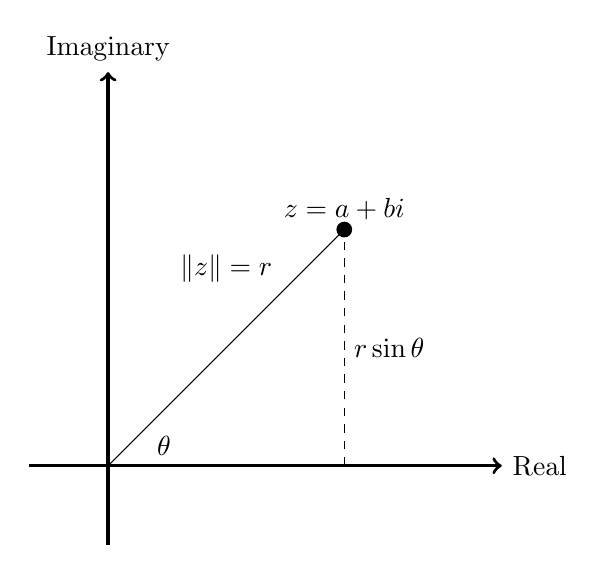
\begin{tikzpicture}
    \draw[very thick,->] (-1,0) -- (5,0) node[right] {Real};
    \draw[very thick,->] (0,-1) -- (0,5) node[above] {Imaginary};
    \draw (0,0) -- (3,3) node[pos=0.5,yshift=1cm] {\( \|z\| = r \)};
    \draw[dashed] (3,0) -- (3,3) node[pos=0.5,right] {\( r\sin\theta \)};
    \fill (3,3) circle[radius=0.1cm] node[above] {\( z = a+bi \)};
    \node[above right] at (0.5,0) {\( \theta \)};
  \end{tikzpicture}
\end{center}
\begin{align*}
  z &= a+bi \\
  &= r\cos\theta+ir\sin\theta, \quad -\pi<\theta<\pm
\end{align*}
Example:
\begin{align*}
  z &= 1+i \\
  \theta &= \frac{\pi}{4} \\
  1+i &= \sqrt{2}\cos(\frac{\pi}{4})+i\sqrt{2}\sin(\frac{\pi}{4})
\end{align*}
Example:
\begin{align*}
  w &= 1-\sqrt{3}i \\
  \theta &= -\frac{\pi}{3} \quad r = \sqrt{4} = 2 \\
  1-\sqrt{3}i &= 2\cos(-\frac{\pi}{3})+i2\sin(-\frac{\pi}{3})
\end{align*}
Polar form is useful because multiplication of complex numbers is much easier in
polar form.
\begin{align*}
  z &= r(\cos\theta+i\sin\theta) \\
  w &= \rho(\cos\phi+i\sin\phi) \\
  zw &= r\rho\left[\cos\theta\cos\phi+i\cos\theta\sin\phi+i\sin\theta\cos\phi+
    i^2\sin\theta\sin\phi\right] \\
  &= r\rho\left[\cos\theta\cos\phi-\sin\theta\sin\phi+
    i(\cos\theta\sin\phi+\sin\theta\cos\phi)\right] \\
  &= r\rho\left[\cos(\theta+\phi)+i\sin(\theta+\phi)\right] \\
  \frac{z}{w} &= \frac{r}{\rho}\left[\cos(\theta-\phi)+i\sin(\theta-\phi)\right]
\end{align*}
Example:
\begin{align*}
  z &= 1+i \\
  &= \sqrt{2}\left(\cos(\frac{\pi}{4})+i\sin(\frac{\pi}{4})\right) \\
  w &= i \\
  &= 1\left(\cos(\frac{\pi}{2})+i\sin(\frac{\pi}{2})\right) \\
  zw &= \sqrt{2}\left[\cos(\frac{3\pi}{4})+i\sin(\frac{3\pi}{4})\right] \\
  &= -1+i
\end{align*}

\subsection*{DeMoivre's Theorem}
Let \( z = r(\cos\theta+i\sin\theta) \):
\begin{align*}
  z^n &= r^n(\cos(n\theta)+i\sin(n\theta)) \\
  z^{\frac{1}{n}} &= r^{\frac{1}{n}}\left[
    \cos\left(\frac{\theta+2k\pi}{n}\right)+
    i\sin\left(\frac{\theta+2k\pi}{n}\right)\right] \quad k = 0,1,\dots,n-1
\end{align*}
Example: Find the three cube roots of \( -27 = 27(\cos\pi+i\sin\pi) \).
\begin{align*}
  (-27)^3 &= 27^{\frac{1}{3}}\left[\cos\left(\frac{\pi+2k\pi}{3}\right)+
    i\sin\left(\frac{\pi+2k\pi}{3}\right)\right] \quad k = 0,1,2 \\
  k &= 0: 3\left[\cos\frac{\pi}{3}+i\sin\frac{\pi}{3}\right] \\
  k &= 1: 3\left[\cos\pi+i\sin\pi\right] \\
  k &= 2: 3\left[\cos\frac{5\pi}{3}+i\sin\frac{5\pi}{3}\right]
\end{align*}

\begin{center}
  You can find all my notes at \url{http://omgimanerd.tech/notes}. If you have
  any questions, comments, or concerns, please contact me at
  alvin@omgimanerd.tech
\end{center}

\end{document}
